\documentclass{ximera}

%\usepackage{todonotes}

\newcommand{\todo}{}

\usepackage{esint} % for \oiint
\ifxake%%https://math.meta.stackexchange.com/questions/9973/how-do-you-render-a-closed-surface-double-integral
\renewcommand{\oiint}{{\large\bigcirc}\kern-1.56em\iint}
\fi


\graphicspath{
  {./}
  {ximeraTutorial/}
  {basicPhilosophy/}
  {functionsOfSeveralVariables/}
  {normalVectors/}
  {lagrangeMultipliers/}
  {vectorFields/}
  {greensTheorem/}
  {shapeOfThingsToCome/}
  {dotProducts/}
  {partialDerivativesAndTheGradientVector/}
  {../productAndQuotientRules/exercises/}
  {../normalVectors/exercisesParametricPlots/}
  {../continuityOfFunctionsOfSeveralVariables/exercises/}
  {../partialDerivativesAndTheGradientVector/exercises/}
  {../directionalDerivativeAndChainRule/exercises/}
  {../commonCoordinates/exercisesCylindricalCoordinates/}
  {../commonCoordinates/exercisesSphericalCoordinates/}
  {../greensTheorem/exercisesCurlAndLineIntegrals/}
  {../greensTheorem/exercisesDivergenceAndLineIntegrals/}
  {../shapeOfThingsToCome/exercisesDivergenceTheorem/}
  {../greensTheorem/}
  {../shapeOfThingsToCome/}
  {../separableDifferentialEquations/exercises/}
}

\newcommand{\mooculus}{\textsf{\textbf{MOOC}\textnormal{\textsf{ULUS}}}}

\usepackage{tkz-euclide}\usepackage{tikz}
\usepackage{tikz-cd}
\usetikzlibrary{arrows}
\tikzset{>=stealth,commutative diagrams/.cd,
  arrow style=tikz,diagrams={>=stealth}} %% cool arrow head
\tikzset{shorten <>/.style={ shorten >=#1, shorten <=#1 } } %% allows shorter vectors

\usetikzlibrary{backgrounds} %% for boxes around graphs
\usetikzlibrary{shapes,positioning}  %% Clouds and stars
\usetikzlibrary{matrix} %% for matrix
\usepackage{pgfplots}
\usepgfplotslibrary{polar} %% for polar plots
\usepgfplotslibrary{fillbetween} %% to shade area between curves in TikZ
\usetkzobj{all}
\usepackage[makeroom]{cancel} %% for strike outs
%\usepackage{mathtools} %% for pretty underbrace % Breaks Ximera
%\usepackage{multicol}
\usepackage{pgffor} %% required for integral for loops



%% http://tex.stackexchange.com/questions/66490/drawing-a-tikz-arc-specifying-the-center
%% Draws beach ball
\tikzset{pics/carc/.style args={#1:#2:#3}{code={\draw[pic actions] (#1:#3) arc(#1:#2:#3);}}}



\usepackage{array}
\setlength{\extrarowheight}{+.1cm}
\newdimen\digitwidth
\settowidth\digitwidth{9}
\def\divrule#1#2{
\noalign{\moveright#1\digitwidth
\vbox{\hrule width#2\digitwidth}}}





\newcommand{\RR}{\mathbb R}
\newcommand{\R}{\mathbb R}
\newcommand{\N}{\mathbb N}
\newcommand{\Z}{\mathbb Z}

\newcommand{\sagemath}{\textsf{SageMath}}


%\renewcommand{\d}{\,d\!}
\renewcommand{\d}{\mathop{}\!d}
\newcommand{\dd}[2][]{\frac{\d #1}{\d #2}}
\newcommand{\pp}[2][]{\frac{\partial #1}{\partial #2}}
\renewcommand{\l}{\ell}
\newcommand{\ddx}{\frac{d}{\d x}}

\newcommand{\zeroOverZero}{\ensuremath{\boldsymbol{\tfrac{0}{0}}}}
\newcommand{\inftyOverInfty}{\ensuremath{\boldsymbol{\tfrac{\infty}{\infty}}}}
\newcommand{\zeroOverInfty}{\ensuremath{\boldsymbol{\tfrac{0}{\infty}}}}
\newcommand{\zeroTimesInfty}{\ensuremath{\small\boldsymbol{0\cdot \infty}}}
\newcommand{\inftyMinusInfty}{\ensuremath{\small\boldsymbol{\infty - \infty}}}
\newcommand{\oneToInfty}{\ensuremath{\boldsymbol{1^\infty}}}
\newcommand{\zeroToZero}{\ensuremath{\boldsymbol{0^0}}}
\newcommand{\inftyToZero}{\ensuremath{\boldsymbol{\infty^0}}}



\newcommand{\numOverZero}{\ensuremath{\boldsymbol{\tfrac{\#}{0}}}}
\newcommand{\dfn}{\textbf}
%\newcommand{\unit}{\,\mathrm}
\newcommand{\unit}{\mathop{}\!\mathrm}
\newcommand{\eval}[1]{\bigg[ #1 \bigg]}
\newcommand{\seq}[1]{\left( #1 \right)}
\renewcommand{\epsilon}{\varepsilon}
\renewcommand{\phi}{\varphi}


\renewcommand{\iff}{\Leftrightarrow}

\DeclareMathOperator{\arccot}{arccot}
\DeclareMathOperator{\arcsec}{arcsec}
\DeclareMathOperator{\arccsc}{arccsc}
\DeclareMathOperator{\si}{Si}
\DeclareMathOperator{\scal}{scal}
\DeclareMathOperator{\sign}{sign}


%% \newcommand{\tightoverset}[2]{% for arrow vec
%%   \mathop{#2}\limits^{\vbox to -.5ex{\kern-0.75ex\hbox{$#1$}\vss}}}
\newcommand{\arrowvec}[1]{{\overset{\rightharpoonup}{#1}}}
%\renewcommand{\vec}[1]{\arrowvec{\mathbf{#1}}}
\renewcommand{\vec}[1]{{\overset{\boldsymbol{\rightharpoonup}}{\mathbf{#1}}}}
\DeclareMathOperator{\proj}{\mathbf{proj}}
\newcommand{\veci}{{\boldsymbol{\hat{\imath}}}}
\newcommand{\vecj}{{\boldsymbol{\hat{\jmath}}}}
\newcommand{\veck}{{\boldsymbol{\hat{k}}}}
\newcommand{\vecl}{\vec{\boldsymbol{\l}}}
\newcommand{\uvec}[1]{\mathbf{\hat{#1}}}
\newcommand{\utan}{\mathbf{\hat{t}}}
\newcommand{\unormal}{\mathbf{\hat{n}}}
\newcommand{\ubinormal}{\mathbf{\hat{b}}}

\newcommand{\dotp}{\bullet}
\newcommand{\cross}{\boldsymbol\times}
\newcommand{\grad}{\boldsymbol\nabla}
\newcommand{\divergence}{\grad\dotp}
\newcommand{\curl}{\grad\cross}
%\DeclareMathOperator{\divergence}{divergence}
%\DeclareMathOperator{\curl}[1]{\grad\cross #1}
\newcommand{\lto}{\mathop{\longrightarrow\,}\limits}

\renewcommand{\bar}{\overline}

\colorlet{textColor}{black}
\colorlet{background}{white}
\colorlet{penColor}{blue!50!black} % Color of a curve in a plot
\colorlet{penColor2}{red!50!black}% Color of a curve in a plot
\colorlet{penColor3}{red!50!blue} % Color of a curve in a plot
\colorlet{penColor4}{green!50!black} % Color of a curve in a plot
\colorlet{penColor5}{orange!80!black} % Color of a curve in a plot
\colorlet{penColor6}{yellow!70!black} % Color of a curve in a plot
\colorlet{fill1}{penColor!20} % Color of fill in a plot
\colorlet{fill2}{penColor2!20} % Color of fill in a plot
\colorlet{fillp}{fill1} % Color of positive area
\colorlet{filln}{penColor2!20} % Color of negative area
\colorlet{fill3}{penColor3!20} % Fill
\colorlet{fill4}{penColor4!20} % Fill
\colorlet{fill5}{penColor5!20} % Fill
\colorlet{gridColor}{gray!50} % Color of grid in a plot

\newcommand{\surfaceColor}{violet}
\newcommand{\surfaceColorTwo}{redyellow}
\newcommand{\sliceColor}{greenyellow}




\pgfmathdeclarefunction{gauss}{2}{% gives gaussian
  \pgfmathparse{1/(#2*sqrt(2*pi))*exp(-((x-#1)^2)/(2*#2^2))}%
}


%%%%%%%%%%%%%
%% Vectors
%%%%%%%%%%%%%

%% Simple horiz vectors
\renewcommand{\vector}[1]{\left\langle #1\right\rangle}


%% %% Complex Horiz Vectors with angle brackets
%% \makeatletter
%% \renewcommand{\vector}[2][ , ]{\left\langle%
%%   \def\nextitem{\def\nextitem{#1}}%
%%   \@for \el:=#2\do{\nextitem\el}\right\rangle%
%% }
%% \makeatother

%% %% Vertical Vectors
%% \def\vector#1{\begin{bmatrix}\vecListA#1,,\end{bmatrix}}
%% \def\vecListA#1,{\if,#1,\else #1\cr \expandafter \vecListA \fi}

%%%%%%%%%%%%%
%% End of vectors
%%%%%%%%%%%%%

%\newcommand{\fullwidth}{}
%\newcommand{\normalwidth}{}



%% makes a snazzy t-chart for evaluating functions
%\newenvironment{tchart}{\rowcolors{2}{}{background!90!textColor}\array}{\endarray}

%%This is to help with formatting on future title pages.
\newenvironment{sectionOutcomes}{}{}



%% Flowchart stuff
%\tikzstyle{startstop} = [rectangle, rounded corners, minimum width=3cm, minimum height=1cm,text centered, draw=black]
%\tikzstyle{question} = [rectangle, minimum width=3cm, minimum height=1cm, text centered, draw=black]
%\tikzstyle{decision} = [trapezium, trapezium left angle=70, trapezium right angle=110, minimum width=3cm, minimum height=1cm, text centered, draw=black]
%\tikzstyle{question} = [rectangle, rounded corners, minimum width=3cm, minimum height=1cm,text centered, draw=black]
%\tikzstyle{process} = [rectangle, minimum width=3cm, minimum height=1cm, text centered, draw=black]
%\tikzstyle{decision} = [trapezium, trapezium left angle=70, trapezium right angle=110, minimum width=3cm, minimum height=1cm, text centered, draw=black]


\outcome{Implicitly differentiate expressions.}
\outcome{Find the equation of the tangent line for curves that
  are not plots of functions.}
\outcome{Understand how changing the variable changes how we take
  the derivative.}
\outcome{Understand the derivatives of expressions that are not
  functions or not ``solved for $y$''.}

\title[Dig-In:]{Implicit differentiation}

\begin{document}
\begin{abstract}
In this section we differentiate equations that contain more than one variable on one side.
\end{abstract}
\maketitle
\section{Review of the chain rule}

Implicit differentiation is really just an application of the chain rule.
So recall:

\begin{theorem}[Chain Rule]\index{chain rule}\index{derivative rules!chain}
If $f(x)$ and $g(x)$ are differentiable, then
\[
\ddx f(g(x)) = f'(g(x))g'(x).
\]
\end{theorem}

Of particular use in this section is the following.  
If $y$ is a differentiable function of $x$ and if $f$ is a differentiable function, then
\[
\ddx (f(y)) = f'(y) \cdot \ddx (y) = f'(y) \dd[y]{x}.
\]


\section{Implicit differentiation}

The functions we've been dealing with so far have been
defined \textit{explicitly}
 in terms of the independent
variable. For example:
\[
y=3x^2-2x+1,\qquad y=e^{3x}, \qquad y = \frac{x-2}{x^2-3x+2}.
\]
However, this is not always  necessary or even possible to do. Sometimes we choose to or we have to define a function  \textit{implicitly
 }. In this case, the dependent variable is not stated
explicitly in terms of an independent variable. Some examples are:
\[
x^2+y^2 = 4,\qquad x^3+y^3 = 9xy, \qquad x^4+3x^2 = x^{2/3}+y^{2/3} + 1.
\]
Your inclination might be simply to solve each of these equations for $y$ and go
merrily on your way. However, this can be difficult or even impossible to do.
%one needs both $y= \sqrt{4-x^2}$ and $y=-\sqrt{4-x^2}$. Moreover, it
%may not even be possible to solve for $y$. 
Since we are often faced with a problem of computing derivatives of such functions,
we need a  method that will enable us to compute derivatives of implicitly defined functions.
% we use \index{implicit differentiation}\textit{implicit
  %differentiation}. 
  
  
  We'll start with a basic example.
  \begin{example}
Consider the curve (a circle) defined by:
\[
x^2 + y^2 = 1
\]
\begin{enumerate}

\item Find the slope of the line tangent to the circle at the point $\left(\frac{\sqrt{2}}{2},\frac{\sqrt{2}}{2}\right)$.
\begin{explanation}
\begin{image}
    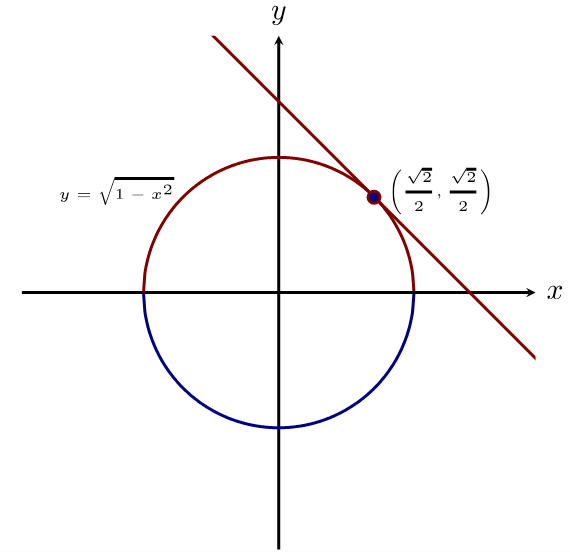
\includegraphics{0.png}
\end{image}

The curve defined by the equation  $x^2 + y^2 = 1$ is not a graph of a function. If we solve for $y$, we obtain two solutions:
$y=\sqrt{1-x^2}$ and $y=-\sqrt{1-x^2}$. 
The point $\left(\frac{\sqrt{2}}{2},\frac{\sqrt{2}}{2}\right)$ lies on the graph of the function $f(x)=\sqrt{1-x^2}$.
Let's compute the derivative of $f$.
\[
f'(x)=\frac{\answer{-2x}}{2\sqrt{1-x^2}}
\]
Therefore, the slope of the tangent line at the point $\left(\frac{\sqrt{2}}{2},\frac{\sqrt{2}}{2}\right)$ is given by
\[
\text{slope}=f'\left(\frac{\sqrt{2}}{2}\right)=\answer{-1}
\]
  \end{explanation}
\item Find the slope of the line tangent to the circle at the point $\left(\frac{\sqrt{2}}{2},-\frac{\sqrt{2}}{2}\right)$.

\begin{explanation}
\begin{image}
      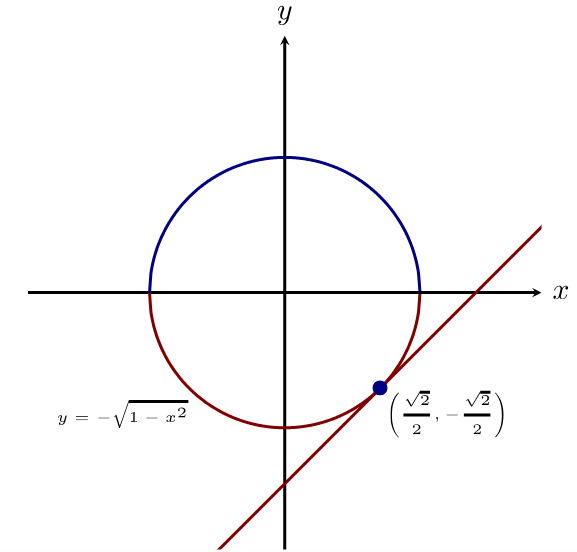
\includegraphics{1.png}
\end{image}
The curve defined by the equation  $x^2 + y^2 = 1$ is not a graph of a function. If we solve for $y$, we obtain two solutions:
$y=\sqrt{1-x^2}$ and $y=-\sqrt{1-x^2}$. 
The point $\left(\frac{\sqrt{2}}{2},-\frac{\sqrt{2}}{2}\right)$ lies on the graph of the function $f(x)=-\sqrt{1-x^2}$.
Let's compute the derivative of $f$.
\[
f'(x)=\frac{\answer{2x}}{2\sqrt{1-x^2}}
\]
Therefore, the slope of the tangent line at the point $\left(\frac{\sqrt{2}}{2},-\frac{\sqrt{2}}{2}\right)$ is given by
\[
\text{slope}=f'\left(\frac{\sqrt{2}}{2}\right)=\answer{1}
\]

Notice that we had to differentiate twice, not to mention that we had to first solve for $y$ in terms of $x$ in order to compute these two slopes.
\end{explanation}
\end{enumerate}
\end{example}
Let's take a different approach, namely let's use implicit differentiation.
\begin{example}
Consider the curve (a circle) defined by:
\[
x^2 + y^2 = 1
\]
\begin{enumerate}
\item Compute $\dd[y]{x}$.
\item Find the slope of the line tangent to the circle at $\left(\frac{\sqrt{2}}{2},\frac{\sqrt{2}}{2}\right)$.
\item Find the slope of the line tangent to the circle at $\left(\frac{\sqrt{2}}{2},-\frac{\sqrt{2}}{2}\right)$.
\end{enumerate}
\begin{explanation}

The curve defined by the equation  $x^2 + y^2 = 1$ is not a graph of a function. If we solve for $y$, we obtain two solutions:
$y=\sqrt{1-x^2}$ and $y=-\sqrt{1-x^2}$. Therefore, we can say that  any point $(x,y)$ on the curve lies on the graph of some function $f$.
  Starting with 
\[
x^2 + y^2 = 1
\]
we differentiate both sides of the
equation with respect to $x$ to obtain
\[
\ddx \left(x^2+y^2\right) = \ddx 1.
\]
Applying the sum rule we see
\[
\ddx x^2+\ddx y^2 = 0.
\]
Let's examine each of these terms in turn. To start
\[
\ddx x^2 = \answer[given]{2x}.
\]
On the other hand, $\ddx y^2$ is somewhat different. Here we assume that $y = f(x)$ for some function $f$, defined on some open interval (this is true for all points $-1<x<1$). Hence, by the chain rule
\begin{align*}
\ddx y^2 &= \ddx (f(x))^2 \\ 
&= 2\cdot f(x) \cdot f'(x) \\
&= 2y\dd[y]{x}.
\end{align*}
Putting this together, we are left with the equation
\[
2x + 2y\dd[y]{x} =0
\]
At this point, we solve for $\dd[y]{x}$. Write
\begin{align*}
2x + 2y\dd[y]{x} &= 0\\
2y \dd[y]{x} &= -2x\\
\dd[y]{x} &= \answer[given]{\frac{-x}{y}}.
\end{align*}
Remark: Notice that the derivative $\dd[y]{x} $ is expressed in terms of both variables $x$ and $y$. This should not come as a surprise. If you think about it, the function and  its derivative are not determined solely by the value of $x$. Recall what happens if $x=\frac{\sqrt{2}}{2}$.


\begin{image}
   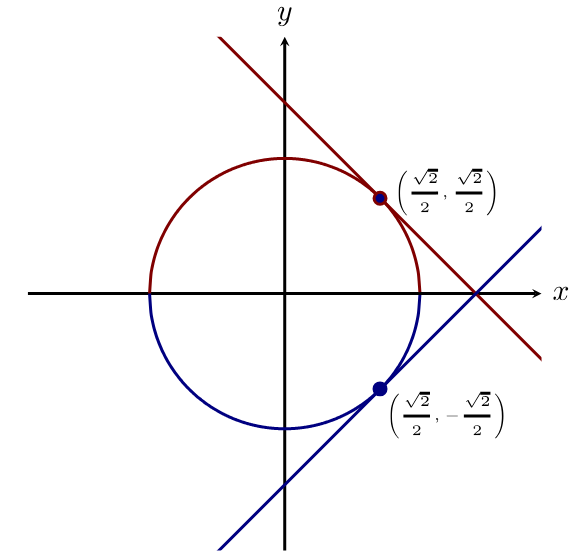
\includegraphics{2.png}
\end{image}
    There are two different points on the curve with  the $x-$coordinate $x=\frac{\sqrt{2}}{2}$.
     
    The advantage of the expression for $\dd[y]{x} $ that we obtained above is that it can be used for computation of the slope of the tangent line at each of these two points, and at any other point on the curve, where defined.
  
 
So, for the second part of the problem, we simply plug $x=\frac{\sqrt{2}}{2}$ and $y=\frac{\sqrt{2}}{2}$
into the expression above, hence the slope of the tangent line at this point 
is $\answer[given]{-1}$.
For the third part of the problem, we simply plug $x=\frac{\sqrt{2}}{2}$ and $y=-\frac{\sqrt{2}}{2}$
into the expression above, hence the slope of the tangent line at this point 
is $\answer[given]{1}$.


\begin{onlineOnly}
  We can confirm our results by looking at the graph of the curve and
  our tangent line:
  \[
  \graph{x^2+y^2=1,-x+\sqrt{2}}
  \]
\end{onlineOnly}
\end{explanation}
\end{example}

Let's see another illustrative example:


\begin{example}
Consider the curve defined by:
\[
x^3+y^3 = 9xy
\]
\begin{image}
  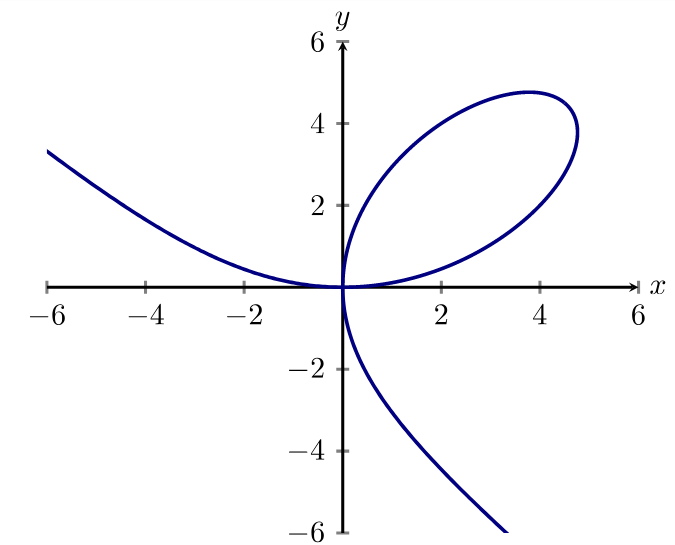
\includegraphics{3.png}
%% \caption{A plot of $x^3+y^3 = 9xy$. While this is not a function of
%%   $y$ in terms of $x$, the equation still defines a relation between
%%   $x$ and $y$.}
\end{image}
\begin{enumerate}
\item Compute $\dd[y]{x}$.
\item Find the slope of the line  tangent to this curve at $(4,2)$.
\end{enumerate}



\begin{explanation}
Starting with 
\[
x^3+y^3 = 9xy,
\]
we differentiate both sides of the
equation with respect to $x$ to obtain
\[
\ddx \left(x^3+y^3\right) = \ddx 9xy.
\]
Applying the sum rule we get that
\[
\ddx x^3+\ddx y^3 = \ddx 9xy.
\]
Let's examine each of these terms in turn. To start
\[
\ddx x^3 = \answer[given]{3x^2}.
\]
On the other hand $\ddx y^3$ is somewhat different. Here you assume that $y = f(x)$, on some interval $I$, and hence by the chain rule
\begin{align*}
\ddx y^3 &= \ddx (f(x))^3 \\ 
&= 3(f(x))^2 \cdot f'(x) \\
&= 3y^2\dd[y]{x}.
\end{align*}
Considering the final term $\ddx 9xy$, we assume that $y=f(x)$, on some interval $I$. Hence 
\begin{align*}
\ddx 9xy &= 9\ddx \Bigl(x\cdot f(x)\Bigr) \\
&= 9 \left(x\cdot f'(x) + f(x)\right)\\
&= 9x \dd[y]{x} + 9y.
\end{align*}
Putting this all together we are left with the equation
\[
3x^2 + 3y^2\dd[y]{x} =9x \dd[y]{x} + 9y.
\]
At this point, we solve for $\dd[y]{x}$. Write
\begin{align*}
3x^2 + 3y^2\dd[y]{x} &= 9x \dd[y]{x} + 9y\\
3y^2\dd[y]{x} -  9x \dd[y]{x} &= 9y - 3x^2\\
\dd[y]{x}\left(3y^2-9x\right)&= 9y - 3x^2\\
\dd[y]{x} &=\frac{9y - 3x^2}{3y^2-9x} = \frac{3y - x^2}{y^2-3x}.
\end{align*}

For the second part of the problem, we simply plug $x=4$ and $y=2$
into the formula above, hence the slope of the tangent line at $(4,2)$
is $\frac{5}{4}$. We've included a plot for your viewing pleasure:
\begin{image}
  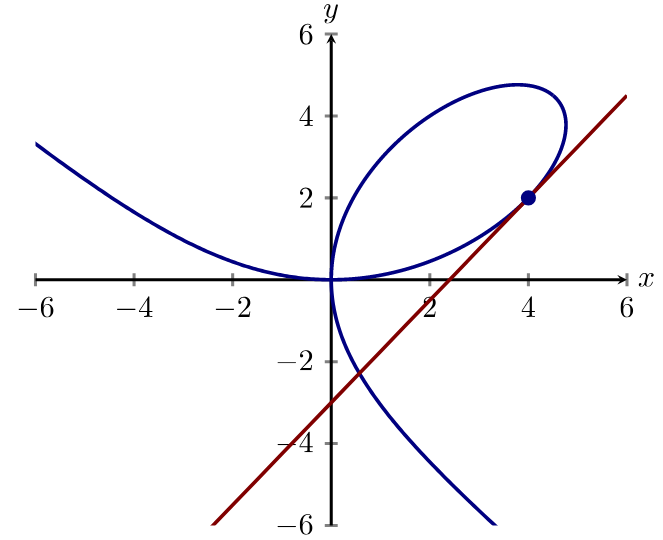
\includegraphics{4.png}
%% \caption{A plot of $x^3+y^3 = 9xy$ along with the tangent line at
%%   $(4,2)$.}
%% \label{plot:x^3+y^3=9xy}
\end{image}
\end{explanation}

\end{example}


You might think that the step in which we solve for $\dd[y]{x}$ could
sometimes be difficult. In fact, \textit{this never happens}. All
occurrences $\dd[y]{x}$ arise from applying the chain rule, and
whenever the chain rule is used it deposits a single $\dd[y]{x}$
multiplied by some other expression. Hence our expression is linear in
$\dd[y]{x}$, it will always be possible to group the terms containing
$\dd[y]{x}$ together and factor out the $\dd[y]{x}$, just as in the
previous examples.

One more last example:

\begin{example}
Consider the curve defined by
\[
\cos(xy) - \frac{y}{x} = 4x^2 y^3.
\]
Compute $\dd[x]{y}$.
\begin{explanation}
First, notice that the problem asks for $\dd[x]{y}$, \textbf{not}
$\dd[y]{x}$. This
means the variables have changed places!  Not to worry, everything is
exactly the same.  We apply $\dd{y}$ to both sides of the equation to
get
\[
\dd{y} \left( \cos(xy) - \frac{y}{x} \right) = \dd{y} (4x^2 y^3)
\]
which gives us
\[
-\answer[given]{\sin(xy)} \left(y \dd[x]{y} + x \right) - \frac{x - y \dd[x]{y}}{x^2}
= 8xy^3 \dd[x]{y} + 12 x^2 y^2.
\]
Distributing and multiplying by $x^2$ yields
\begin{align*}
  -x^2 y \sin(xy) \dd[x]{y} &- x^3 \sin(xy) - x + y \dd[x]{y}\\
  &= 8x^3y^3 \dd[x]{y} + 12x^4y^2.
\end{align*}
Grouping terms, factoring, and dividing finally gives us
\begin{align*}
  -x^2 y \sin(xy) \dd[x]{y} &+ y \dd[x]{y} - 8x^3y^3 \dd[x]{y} \\
  &= x^3 \sin(xy) + x + 12x^4 y^2
\end{align*}
so,
\[
\left( y - x^2y\sin(xy) - 8x^3 y^3 \right) \dd[x]{y} = x^3 \sin(xy) + x + 12x^4 y^2 
\]
and now we see
\[
\dd[x]{y} = \frac{x^3 \sin(xy) + x + 12x^4 y^2}{y - x^2y\sin(xy) - 8x^3 y^3}.
\]
\end{explanation}
\end{example}
\end{document}